\hypertarget{_metacommunity_8cpp}{}\section{necsim/\+Metacommunity.cpp File Reference}
\label{_metacommunity_8cpp}\index{necsim/\+Metacommunity.\+cpp@{necsim/\+Metacommunity.\+cpp}}


Contains the \hyperlink{class_metacommunity}{Metacommunity} class for generating a neutral metacommunity.  


{\ttfamily \#include \char`\"{}Metacommunity.\+h\char`\"{}}\\*
Include dependency graph for Metacommunity.\+cpp\+:\nopagebreak
\begin{figure}[H]
\begin{center}
\leavevmode
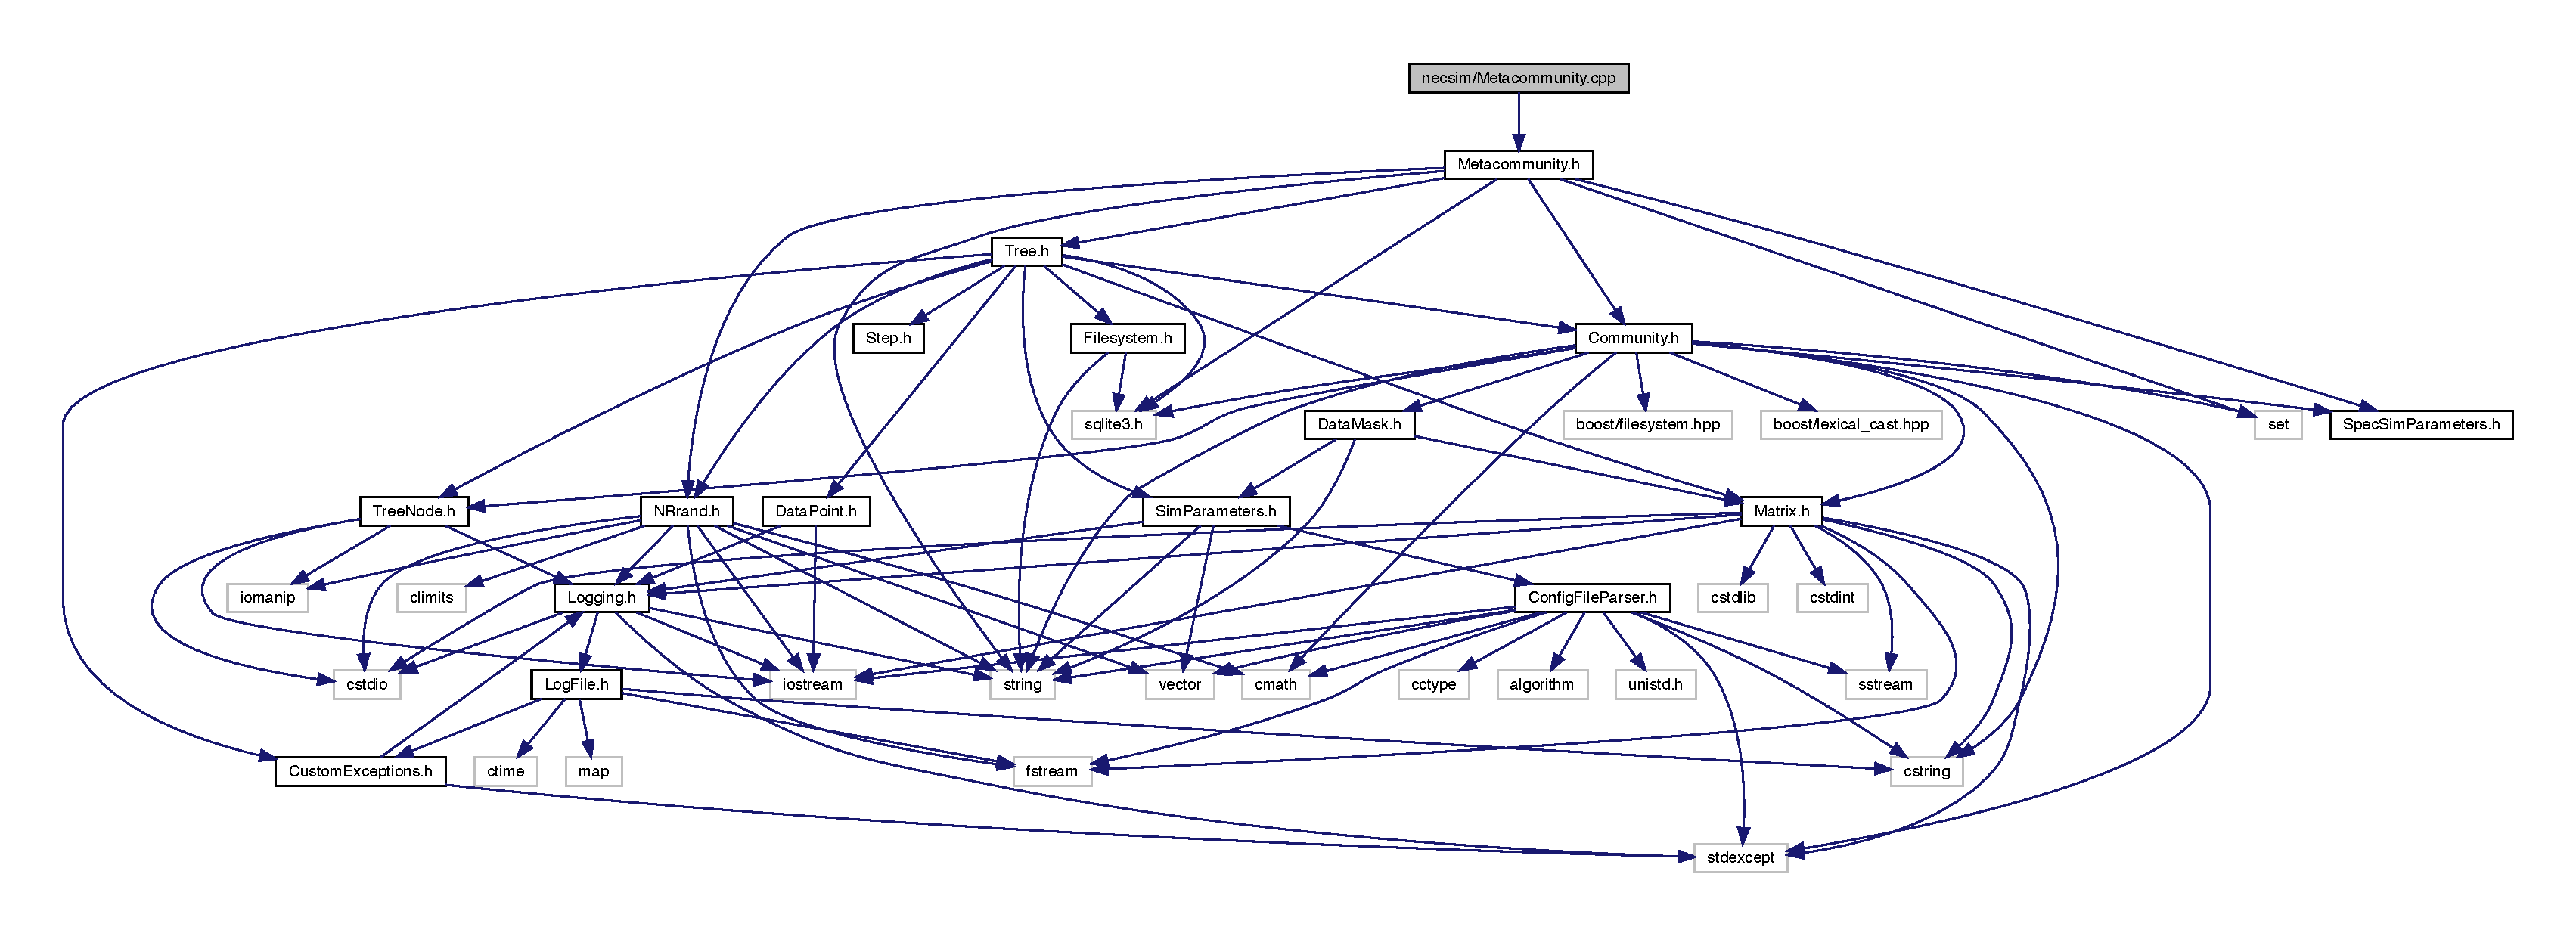
\includegraphics[width=350pt]{_metacommunity_8cpp__incl}
\end{center}
\end{figure}


\subsection{Detailed Description}
Contains the \hyperlink{class_metacommunity}{Metacommunity} class for generating a neutral metacommunity. 

\begin{DoxyAuthor}{Author}
Samuel Thompson
\end{DoxyAuthor}
\begin{DoxyCopyright}{Copyright}
\href{https://opensource.org/licenses/BSD-3-Clause}{\tt B\+S\+D-\/3 Licence.} For use with completed simulations from N\+E\+C\+Sim, using the Speciation\+Counter program. Individuals will be drawn from the metacommunity for each speciation event, instead of creating a new species each time.
\end{DoxyCopyright}
Contact\+: \href{mailto:samuel.thompson14@imperial.ac.uk}{\tt samuel.\+thompson14@imperial.\+ac.\+uk} or \href{mailto:thompsonsed@gmail.com}{\tt thompsonsed@gmail.\+com} 